\documentclass[11pt, a4paper]{article}

% Pacchetti base per lingua e codifica
\usepackage[utf8]{inputenc}
\usepackage[italian]{babel}

% Pacchetti per la matematica e la fisica
\usepackage{amsmath, amssymb, amsfonts}
\usepackage{cancel} % Utile per sbarrare i termini che si annullano

% Pacchetti per la grafica e l'impaginazione
\usepackage{graphicx}
\usepackage{geometry}
\geometry{top=2.5cm, bottom=2.5cm, left=2.5cm, right=2.5cm}
\usepackage{booktabs}
\usepackage{multirow}
\usepackage{sectsty}
\usepackage{float}
\usepackage{xcolor}
\allsectionsfont{\underline}
\setcounter{secnumdepth}{0}

\begin{document}
\tableofcontents

\newpage

\section{Richiamo sul Moto Ondulatorio} %

L'equazione generale di un'onda piana armonica è: %
\begin{equation*}
    f(x,t) = \underbrace{A}_{\text{Amp.}} e^{i\overbrace{(kx \pm \omega t)}^{\text{Fase}}} %
\end{equation*}
Il segno determina la direzione di propagazione: %
\begin{itemize}
    \item $\ominus \Rightarrow \text{PROGRESSIVA}$ %
    \item $\oplus \Rightarrow \text{REGRESSIVA}$ %
\end{itemize}
La velocità di propagazione dell'onda è $v = \frac{\omega}{k}$ %.

\begin{figure}[H]
    \centering
    \begin{minipage}{0.3\textwidth}
        \centering
        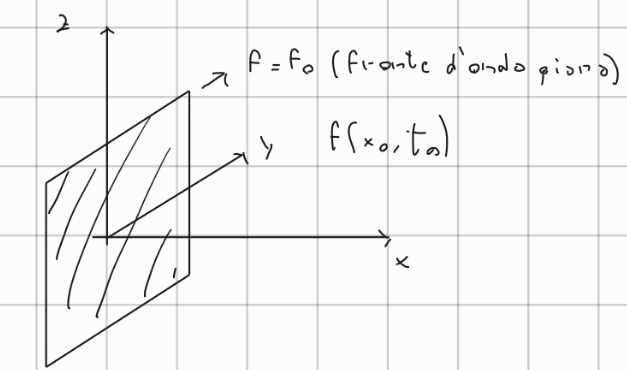
\includegraphics[width=\linewidth]{immagini/2026-03-21-14-38-39.png}
    \end{minipage}\hfill
    \begin{minipage}{0.3\textwidth}
        \centering
        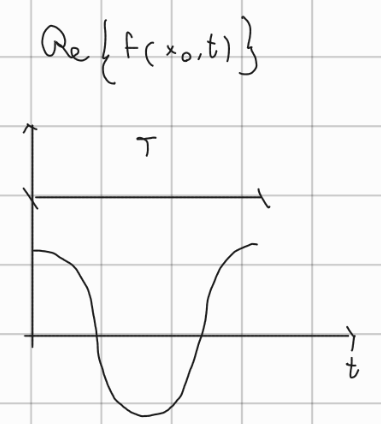
\includegraphics[width=0.8\linewidth]{immagini/2026-03-21-14-38-12.png}
    \end{minipage}\hfill
    \begin{minipage}{0.3\textwidth}
        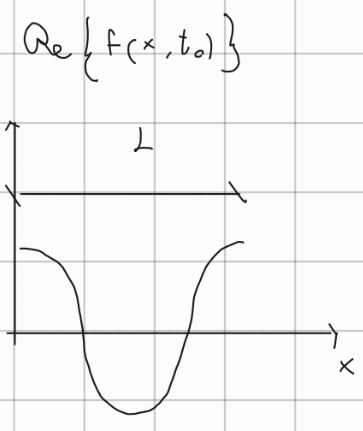
\includegraphics[width=0.8\linewidth]{immagini/2026-03-21-14-37-53.png}
    \end{minipage}
\end{figure}

La relazione fondamentale, fissata dalla sorgente, è: %
\begin{equation}
    \lambda \nu = |\vec{v}| %
\end{equation}

Estensione alle onde in 3 dimensioni (Es. onda sferica): %
\begin{equation*}
    f(\vec{r}, t) = A(r) e^{i(\vec{k}\cdot\vec{r} \pm \omega t)} \quad \text{con } A(r) = \frac{A_0}{r} %
\end{equation*}

\subsection{Onde Reali e Pacchetto d'Onda} %

Le onde reali hanno una lunghezza finita, si definiscono quindi come un \textbf{Pacchetto d'onda} %.
Sovrapponiamo due onde con frequenze e vettori d'onda simili ($\omega_1 \simeq \omega_2$ e $k_1 \simeq k_2$): %
\begin{equation*}
    f(x,t) = f_1(x,t) + f_2(x,t) = A \cos(k_1 x - \omega_1 t) + A \cos(k_2 x - \omega_2 t) %
\end{equation*}

Usando le formule trigonometriche, si ottiene un'onda modulata (\textbf{BATTIMENTI}): %
\begin{equation}
    f(x,t) = A \cos(\Delta k x - \Delta \omega t) \cos(k_m x - \omega_m t) %
\end{equation}
dove le differenze e le medie sono definite come: %
\begin{figure}[H]
    \centering
    \begin{minipage}{0.5\textwidth}
        \centering
        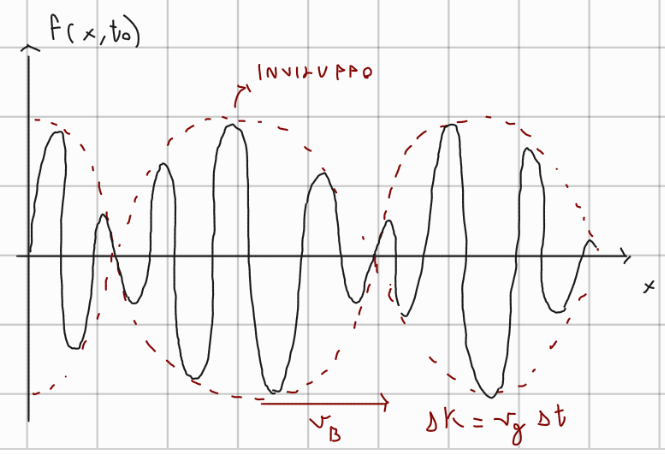
\includegraphics[width=\linewidth]{immagini/2026-03-21-14-41-12.png}
    \end{minipage}\hfill
    \begin{minipage}{0.5\textwidth}
        \begin{align*}
            \Delta \omega &= \frac{\omega_1 - \omega_2}{2} & \omega_m &= \frac{\omega_1 + \omega_2}{2} \\ %
            \Delta k &= \frac{k_1 - k_2}{2} & k_m &= \frac{k_1 + k_2}{2} %
        \end{align*}
    \end{minipage}
\end{figure}

Per un pacchetto d'onda si definiscono due velocità distinte: %
\begin{itemize}
    \item $v_f$ (\textbf{velocità di fase}) $= \frac{\omega_m}{k_m}$ (è la velocità delle creste interne) %.
    \item $v_g$ (\textbf{velocità di gruppo}) $= \frac{\Delta \omega}{\Delta k}$ (è la velocità con cui trasla l'inviluppo, ovvero l'energia) %.
\end{itemize}

\noindent
A seconda di come si propaga l'onda, un mezzo si divide in: %
\begin{itemize}
    \item \textbf{NON DISPERSIVO:} se $v_f = v_g$ %
    \item \textbf{DISPERSIVO:} se $v_f \neq v_g$ %
\end{itemize}

\noindent
Generalizzando la sovrapposizione a infinite frequenze, un pacchetto si scrive tramite un integrale: %
\begin{equation}
    f(x,t) = \frac{1}{\sqrt{2\pi}} \int_{-\infty}^{+\infty} A(k) e^{i(kx - \omega t)} \, dk %
\end{equation}
$\Rightarrow$ Questo rappresenta una somma di onde piane armoniche, ognuna pesata con la sua ampiezza $A(k)$ %.

Se il mezzo non assorbe, valutando all'istante $t=0$, troviamo: %
\begin{equation}
    A(k) = \frac{1}{\sqrt{2\pi}} \int_{-\infty}^{+\infty} f(x,0) e^{-ikx} \, dx \quad \Rightarrow \quad \textbf{TRASFORMATA DI FOURIER} %
\end{equation}

Passando al continuo con il limite differenziale: %
\begin{equation*}
    v_f = \frac{\omega_n}{k_n} \quad , \quad v_g = \lim_{\Delta k \to 0} \frac{\Delta \omega}{\Delta k} = \frac{d\omega}{dk} %
\end{equation*}
La funzione $\omega = \omega(k)$ è chiamata \textbf{RELAZIONE DI DISPERSIONE} %.
$\hookrightarrow$ In un mezzo non dispersivo si ha una relazione lineare: $\omega = ck \Rightarrow v_g = c$ %.

\subsection{Esempio: Trasformata di un'onda confinata} %

Consideriamo una funzione d'onda troncata, esistente solo in una regione di larghezza $L$: %
\begin{figure}[H]
    \centering
    \begin{minipage}{0.3\textwidth}
        \centering
        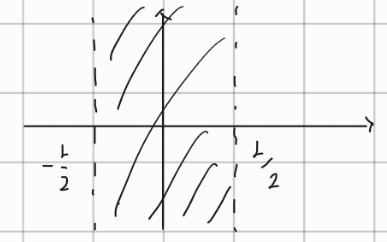
\includegraphics[width=\linewidth]{immagini/2026-03-21-14-45-24.png}
    \end{minipage}\hfill
    \begin{minipage}{0.65\textwidth}
        \begin{equation*}
            f(x,0) = \begin{cases}
                c e^{i k_0 x} & -\frac{L}{2} < x < \frac{L}{2} \\ %
                0 & \text{Altrove} %
            \end{cases}
        \end{equation*}
    \end{minipage}
\end{figure}

Calcoliamo l'ampiezza spettrale $A(k)$ con l'integrale di Fourier: %
\begin{figure}[H]
    \centering
    \begin{minipage}{0.3\textwidth}
        \centering
        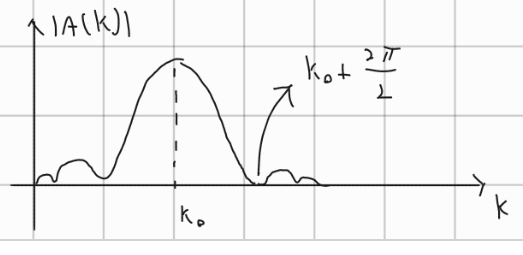
\includegraphics[width=\linewidth]{immagini/2026-03-21-14-45-59.png}
    \end{minipage}\hfill
    \begin{minipage}{0.65\textwidth}
        \begin{align*}
            A(k) &= \frac{1}{\sqrt{2\pi}} \int_{-L/2}^{L/2} c e^{i k_0 x} e^{-i k x} \, dx = \frac{c}{\sqrt{2\pi}} \int_{-L/2}^{L/2} e^{i(k_0 - k)x} \, dx = \\ %
                 &= \frac{c}{\sqrt{2\pi}} \left[ \frac{e^{i(k_0 - k)x}}{i(k_0 - k)} \right]_{-L/2}^{L/2} = \frac{c}{\sqrt{2\pi}} \left[ \frac{e^{i(k_0 - k)\frac{L}{2}} - e^{-i(k_0 - k)\frac{L}{2}}}{i(k_0 - k)} \right] = \\ %
                 &= \frac{2c}{\sqrt{2\pi}} \frac{\sin\left[(k_0 - k)\frac{L}{2}\right]}{k_0 - k} \quad \text{(\textit{Seno cardinale})} %
        \end{align*}
    \end{minipage}
\end{figure}

\textbf{Osservazione (Preludio al Principio di Indeterminazione):} %
\begin{itemize}
    \item Se $L \to +\infty$ (onda infinita), gli zeri della funzione \textit{sinc} si schiacciano su $k \rightarrow$ si torna ad avere un'onda monocromatica formata da un solo vettore d'onda $K$ %.
    \item Al contrario, \textbf{più il pacchetto dura poco} nello spazio (piccolo $L$), \textbf{più devo considerare tante frequenze} (ovvero tanti $k$) per poterlo generare %.
\end{itemize}

\section{Esperimento di Young (Interferenza da 2 fenditure)} %

Consideriamo un'onda piana incidente su due fenditure distanti $d$. La luce viaggia verso uno schermo posto a distanza $L \to \infty$ (raggi paralleli) %. 
La differenza di cammino ottico tra i due raggi per raggiungere il punto $P$ sotto un angolo $\theta$ è: %
\begin{equation*}
    r_2 - r_1 = d \sin\theta %
\end{equation*}

I campi elettrici delle due onde nel punto $P$ sono: %
\begin{figure}[H]
    \centering
    \begin{minipage}{0.3\textwidth}
        \centering
        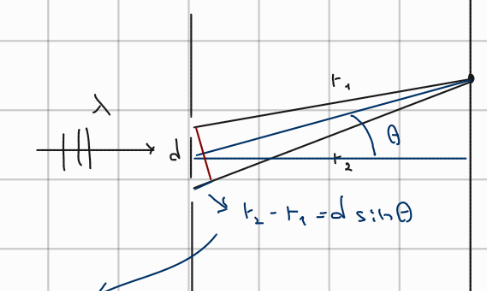
\includegraphics[width=\linewidth]{immagini/2026-03-21-14-49-28.png}
    \end{minipage}\hfill
    \begin{minipage}{0.3\textwidth}
        \begin{align*}
            \mathcal{E}_1(P) &= \mathcal{E}_{01} e^{i(kr_1 - \omega t)} \\ %
            \mathcal{E}_2(P) &= \mathcal{E}_{02} e^{i(kr_2 - \omega t)} %
        \end{align*}
    \end{minipage}
    \begin{minipage}{0.3\textwidth}
        \centering
        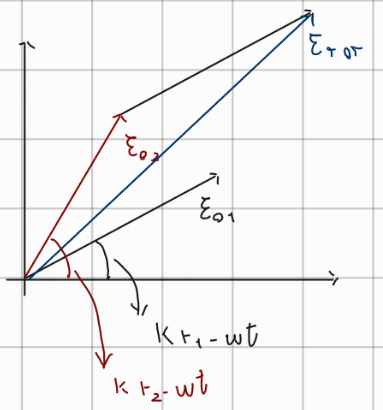
\includegraphics[width=0.8\linewidth]{immagini/2026-03-21-14-49-56.png}
    \end{minipage}\hfill
\end{figure}
Per il principio di sovrapposizione: $\mathcal{E}_{TOT}(P) = \mathcal{E}_1(P) + \mathcal{E}_2(P)$. %


Sommando i fasori, l'ampiezza totale è: %
\begin{equation*}
    \mathcal{E}_{TOT} = \sqrt{\mathcal{E}_{01}^2 + \mathcal{E}_{02}^2 + 2\mathcal{E}_{01}\mathcal{E}_{02}\cos\delta} %
\end{equation*}
dove la differenza di fase (stazionaria nel tempo) è: %
\begin{equation*}
    \delta = (kr_2 - \omega t) - (kr_1 - \omega t) = k(r_2 - r_1) %
\end{equation*}

\noindent
Poiché l'intensità $I(P) \propto |\mathcal{E}_{TOT}(P)|^2$, se le fenditure sono identiche ($\mathcal{E}_{01} = \mathcal{E}_{02} = \mathcal{E}_0$ e $I_1=I_2=I_0$), otteniamo il pattern di interferenza: %
\begin{equation}
    I(P) = I_1 + I_2 + 2\sqrt{I_1 I_2} \cos(k(r_2 - r_1)) = 2I_0(1 + \cos\delta) %
\end{equation}

Troviamo i punti di \textbf{Massimo} e \textbf{Minimo}: %
\begin{itemize}
    \item \textbf{MAX:} $\cos\delta = 1 \Rightarrow k(r_2 - r_1) = 2m\pi \Rightarrow k d \sin\theta = 2m\pi \Rightarrow \boxed{ \sin\theta_{MAX} = m\frac{\lambda}{d} }$ \quad ($m = 0, \pm 1, \pm 2 \dots$) %
    \item \textbf{MIN:} $\cos\delta = -1 \Rightarrow k(r_2 - r_1) = (2m+1)\pi \Rightarrow \boxed{ \sin\theta_{MIN} = (2m+1)\frac{\lambda}{2d} }$ %
\end{itemize}

Posizione lineare dei massimi sullo schermo (approssimazione per piccoli angoli $\sin\theta \simeq \tan\theta = \frac{y}{L}$): %
\begin{figure}[H]
    \centering
    \begin{minipage}{0.3\textwidth}
        \centering
        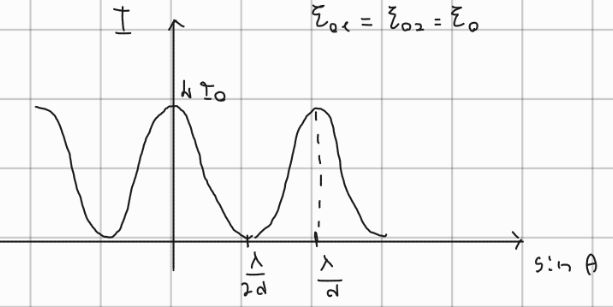
\includegraphics[width=\linewidth]{immagini/2026-03-21-14-51-25.png}
    \end{minipage}\hfill
    \begin{minipage}{0.65\textwidth}
        \begin{equation*}
            y_{max} = m \frac{\lambda L}{d} %
        \end{equation*}
    \end{minipage}
\end{figure}

\subsection{Interferenza da N Sorgenti} %

Generalizzando per $N$ fenditure equidistanti (come in un reticolo), la formula dell'intensità diventa: %
\begin{equation}
    \boxed{ I(\theta) = I_0 \left( \frac{\sin(N\frac{\delta}{2})}{\sin(\frac{\delta}{2})} \right)^2 } \quad \text{con } \delta = k d \sin\theta %
\end{equation}

Analisi dei picchi: %
\begin{enumerate}
    \item \textbf{Massimi Assoluti (Principali):} Il denominatore si annulla, $\sin(\frac{\delta}{2}) = 0 \Rightarrow \frac{\delta}{2} = m\pi \Rightarrow \delta = 2m\pi \Rightarrow \sin\theta_M = m\frac{\lambda}{d}$ %. 
    Risolvendo il limite per $\delta \to 0$ (o multipli): %
    \begin{equation*}
        \lim_{\delta \to 0} \left( \frac{N \frac{\delta}{2}}{\frac{\delta}{2}} \right)^2 = N^2 \quad \Rightarrow \quad \boxed{ I_{MAX} = I_0 N^2 } %
    \end{equation*}
    \item \textbf{Minimi Assoluti:} Il numeratore si annulla ma il denominatore no, $\sin(N\frac{\delta}{2}) = 0 \Rightarrow N\frac{\delta}{2} = m\pi \Rightarrow \delta = 2\frac{m}{N}\pi \Rightarrow \sin\theta_m = m\frac{\lambda}{Nd}$ (con $m \notin \mathbb{Z}^0$, non multiplo di $N$) %.
\end{enumerate}
\textit{Regola:} Tra due massimi principali avrò $N-1$ minimi in cui $I=0$, e avrò $N-2$ \textbf{Massimi Secondari} %.

\section{Diffrazione da Singola Fenditura ($a \simeq \lambda$)} %

Consideriamo una fenditura di larghezza $a$, divisibile in un'infinità di sorgentini secondari $N \to \infty$ distanti $d$ tali che $Nd = a$ (Principio di Huygens-Fresnel). %

\noindent
L'ampiezza totale al centro è $A_0 = N A'$, che corrisponde alla lunghezza dell'arco nel diagramma dei fasori. L'ampiezza all'angolo $\theta$ è la corda sottesa dall'arco:
\begin{figure}[H]
    \centering
    \begin{minipage}{0.3\textwidth}
        \centering
        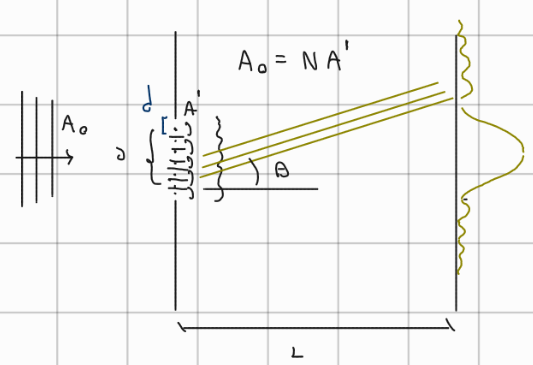
\includegraphics[width=\linewidth]{immagini/2026-03-21-14-57-51.png}
    \end{minipage}\hfill
    \begin{minipage}{0.3\textwidth}
        \centering
        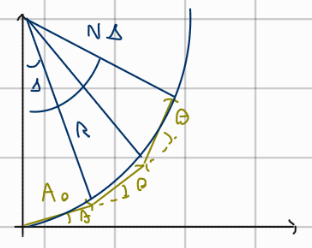
\includegraphics[width=\linewidth]{immagini/2026-03-21-14-56-04.png}
    \end{minipage}\hfill
    \begin{minipage}{0.3\textwidth}
        
        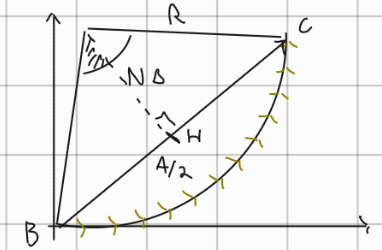
\includegraphics[width=\linewidth]{immagini/2026-03-21-14-55-43.png}
    \end{minipage}
\end{figure}

\begin{equation*}
    A = 2 R \sin\left(\frac{N\delta}{2}\right) \quad \text{e sapendo che} \quad A_0 = R N \delta \Rightarrow R = \frac{A_0}{N\delta} %
\end{equation*}
Sostituendo $R$: %
\begin{equation*}
    A = \frac{A_0}{N\delta/2} \sin\left(\frac{N\delta}{2}\right) = A_0 \, \text{sinc}\left(\frac{N\delta}{2}\right) %
\end{equation*}
Sviluppando l'argomento: $\frac{N\delta}{2} = \frac{N(kd\sin\theta)}{2} = \frac{k(Nd)\sin\theta}{2} = \frac{2\pi a \sin\theta}{2\lambda} = \frac{\pi a}{\lambda}\sin\theta$ %.
La funzione di ampiezza e l'intensità diffratta diventano: %
\begin{figure}[H]
    \centering
    \begin{minipage}{0.3\textwidth}
        \centering
        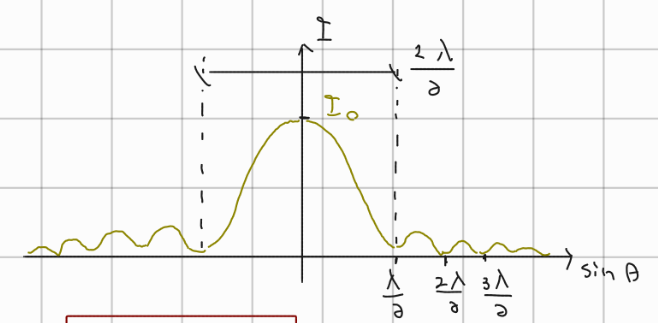
\includegraphics[width=\linewidth]{immagini/2026-03-21-15-14-04.png}
    \end{minipage}\hfill
    \begin{minipage}{0.65\textwidth}
        \begin{equation}
            A = A_0 \, \text{sinc}\left(\frac{\pi a}{\lambda}\sin\theta\right) \quad \Rightarrow \quad \boxed{ I = I_0 \, \text{sinc}^2\left(\frac{\pi a}{\lambda}\sin\theta\right) } %
        \end{equation}
    \end{minipage}
\end{figure}

\noindent
\textbf{Minimi di Diffrazione (Zeri):} %
La funzione sinc si annulla quando l'argomento è un multiplo intero di $\pi$: %
\begin{equation}
    \frac{\pi a}{\lambda} \sin\theta = m\pi \quad \Rightarrow \quad \boxed{ \sin\theta_m = m\frac{\lambda}{a} } \quad (m \in \mathbb{Z}^0) %
\end{equation}

\noindent
\textit{Limiti geometrici:} Affinché lo zero sia visibile sullo schermo, $\sin\theta \le 1 \Rightarrow m\frac{\lambda}{a} \le 1 \Rightarrow m_{MAX} = \lfloor \frac{a}{\lambda} \rfloor$ %. 
\begin{itemize}
    \item Se $a \gg \lambda$, lo spettro "si schiaccia" tutto al centro (ritorno all'ottica geometrica) %.
    \item Se $a \simeq \lambda \Rightarrow m_{MAX} = 1$ (diffrazione estesissima, copre tutto l'angolo) %.
\end{itemize}

\begin{figure}[H]
    \centering
    \begin{minipage}{0.3\textwidth}
        \centering
        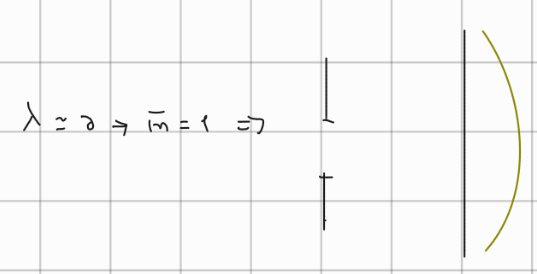
\includegraphics[width=\linewidth]{immagini/2026-03-21-15-17-29.png}
    \end{minipage}\hfill
    \begin{minipage}{0.65\textwidth}
        Per praticamente tutte le applicazioni reali mi ritrovo ad avere una certa quantità di diffrazione
    \end{minipage}
\end{figure}

\section{Reticolo di Diffrazione Completo} %

Un reticolo reale ha $N$ fenditure di larghezza finita $a$, distanti $d$. L'intensità proiettata sullo schermo è il prodotto esatto tra l'\textbf{Inviluppo di Diffrazione} (della singola fenditura) e il \textbf{Pattern di Interferenza} (delle $N$ fenditure): %
\begin{figure}[H]
    \centering
    \begin{minipage}{0.3\textwidth}
        \centering
        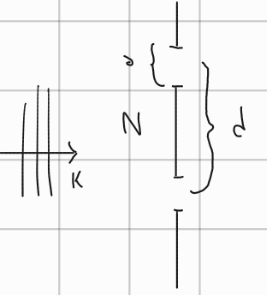
\includegraphics[width=0.7\linewidth]{immagini/2026-03-21-15-18-05.png}
    \end{minipage}\hfill
    \begin{minipage}{0.65\textwidth}
        \begin{equation}
            I = I_0 \underbrace{\left[ \frac{\sin(\frac{\pi a}{\lambda}\sin\theta)}{\frac{\pi a}{\lambda}\sin\theta} \right]^2}_{\text{Diffrazione (Inviluppo)}} \times \underbrace{\left[ \frac{\sin(N\frac{\pi d}{\lambda}\sin\theta)}{\sin(\frac{\pi d}{\lambda}\sin\theta)} \right]^2}_{\text{Interferenza (Picchi)}} %
        \end{equation}
    \end{minipage}
\end{figure}

\begin{figure}[H]
    \centering
    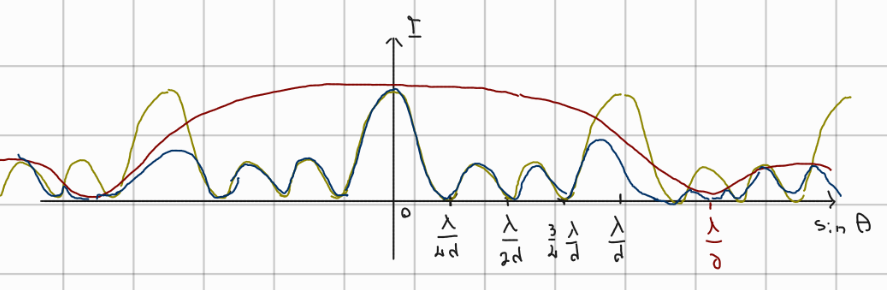
\includegraphics[width=0.6\linewidth]{immagini/2026-03-21-15-18-24.png}
    \end{figure}

\subsection{Diffrazione di Bragg (Cristallografia)} %

I reticoli cristallini sono composti da atomi spaziati regolarmente con passo $d \simeq 10^{-10} \text{ m}$ ($1 \text{\AA}$). Affinché vi sia diffrazione, occorre usare luce con $\lambda \simeq 10^{-10} \text{ m} \Rightarrow$ \textbf{Raggi X} %. 

\noindent
Se un'onda incide sui piani cristallini con angolo $\theta$ (rispetto al piano), la differenza di fase tra la luce riflessa dal primo e dal secondo piano è determinata dalla differenza di cammino geometrico: %
\begin{figure}[H]
    \centering
    \begin{minipage}{0.3\textwidth}
        \centering
        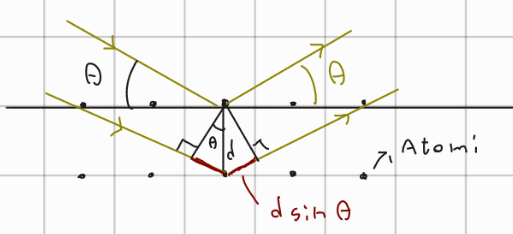
\includegraphics[width=\linewidth]{immagini/2026-03-21-15-19-38.png}
    \end{minipage}\hfill
    \begin{minipage}{0.65\textwidth}
        \begin{equation*}
            \Delta_{fase} = k(2d\sin\theta) %
        \end{equation*}
    \end{minipage}
\end{figure}

Si avrà un massimo di interferenza costruttiva (picco di riflessione) quando la differenza di fase è un multiplo di $2\pi$: %
\begin{equation*}
    MAX \Rightarrow \Delta_{fase} = 2m\pi \quad \Rightarrow \quad \left(\frac{2\pi}{\lambda}\right) 2d\sin\theta = 2m\pi %
\end{equation*}
Semplificando, si ricava la celebre \textbf{Legge di Bragg}: %
\begin{equation}
    \boxed{ \sin\theta_{MAX} = m\frac{\lambda}{2d} } \quad \text{(condizione per i picchi di diffrazione)} %
\end{equation}

\section{Unificazione di Onde e Corpuscoli} %

Cerchiamo di mettere insieme i due mondi (classico e quantistico) per la luce. %
Sappiamo che:
\begin{equation*}
    E = h\nu = \hbar\omega \quad \text{e che l'Intensità } I \propto N^\circ \text{ Fotoni} %
\end{equation*}
L'onda elettromagnetica è descritta dal campo elettrico: $\mathcal{E}(x,t) = \bar{\mathcal{E}} \cos(kx - \omega t)$, a cui associamo l'\textbf{Energia del fotone} %.

\noindent
Ricaviamo la quantità di moto del fotone partendo dall'energia relativistica (con massa a riposo $m=0$): %
\begin{equation*}
    E = \sqrt{p^2 c^2 + m^2 c^4} = pc \quad \Rightarrow \quad E = pc = h\nu \quad \Rightarrow \quad p = \frac{h\nu}{c} = \frac{h}{\lambda} %
\end{equation*}
Sostituendo $k = \frac{2\pi}{\lambda}$ (da cui $\frac{1}{\lambda} = \frac{k}{2\pi}$): %
\begin{equation*}
    p = \frac{h}{2\pi} k = \hbar k \quad \Rightarrow \quad \boxed{ \vec{p} = \hbar \vec{k} } \quad \text{(\textbf{Momento del FOTONE})} %
\end{equation*}

\subsection{Relazione tra Intensità d'Onda e Flusso di Fotoni} %

Classicamente, l'intensità è proporzionale al quadrato dell'ampiezza ($I \propto |\mathcal{E}|^2$). Quantisticamente, è proporzionale al numero di fotoni: %
\begin{equation*}
    I = \mu_{em} c = \varepsilon_0 |\mathcal{E}(x,t)|^2 c \quad \Rightarrow \quad \langle I \rangle = \frac{1}{2} \varepsilon_0 \bar{\mathcal{E}}^2 c = N \cdot \hbar\omega %
\end{equation*}
Analisi dimensionale e definizioni: %
\begin{itemize}
    \item $\langle I \rangle = \left[ \frac{\text{W}}{\text{m}^2} \right] = \left[ \frac{\text{J}}{\text{s} \cdot \text{m}^2} \right]$ (Intensità media) %
    \item $N$: \textbf{Flusso di fotoni} $\left[ \frac{\text{\# fotoni}}{\text{s} \cdot \text{m}^2} \right]$ %
    \item $\hbar\omega$: Energia di un singolo fotone $[\text{J}]$ %
\end{itemize}
Da cui si ricava il numero di fotoni per unità di area e di tempo: %
\begin{equation}
    N = \frac{\varepsilon_0 c \bar{\mathcal{E}}^2}{2 \hbar\omega} = \frac{\langle I \rangle}{\hbar\omega} %
\end{equation}

\noindent
\textbf{Esempio numerico (LASER rosso):} %
Dati: $\hbar\omega = 2 \text{ eV}$, $I = 1 \text{ mW}/\text{mm}^2$. %
\begin{equation*}
    \langle I \rangle = \frac{10^{-3} \text{ W}}{10^{-6} \text{ m}^2} = 10^3 \frac{\text{W}}{\text{m}^2} %
\end{equation*}
Calcoliamo il flusso di fotoni: %
\begin{equation*}
    N = \frac{\langle I \rangle}{\hbar\omega} = \frac{10^3 \text{ J}/(\text{s}\cdot\text{m}^2)}{2 \cdot 1.6 \cdot 10^{-19} \text{ J}} \simeq 3 \cdot 10^{21} \frac{\text{fotoni}}{\text{s} \cdot \text{m}^2} %
\end{equation*}
Calcoliamo il campo elettrico equivalente: %
\begin{equation*}
    \bar{\mathcal{E}} = \sqrt{\frac{N \cdot 2 \hbar\omega}{c \varepsilon_0}} \simeq 850 \frac{\text{V}}{\text{m}} %
\end{equation*}

\section{Dualismo Onda-Particella: La Doppia Fenditura} %

Dall'ottica ondulatoria, sappiamo che per due fenditure ($N=2$): %
\begin{figure}[H]
    \centering
    \begin{minipage}{0.3\textwidth}
        \centering
        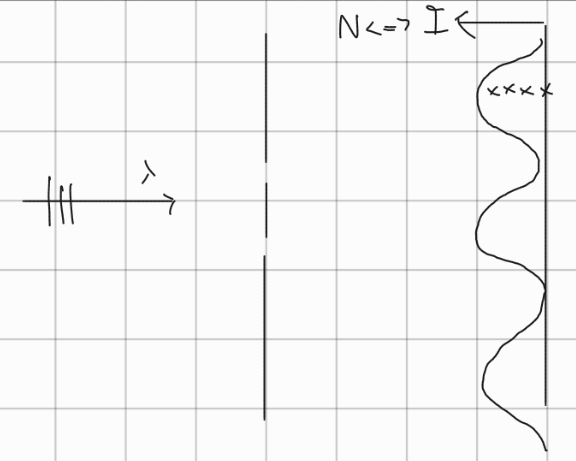
\includegraphics[width=\linewidth]{immagini/2026-03-21-15-23-13.png}
    \end{minipage}\hfill
    \begin{minipage}{0.65\textwidth}
        \begin{equation*}
            I(\theta) = I_0 \left[ \frac{\sin\left(\frac{2\pi d \sin\theta}{\lambda}\right)}{\sin\left(\frac{\pi d \sin\theta}{\lambda}\right)} \right]^2 %
        \end{equation*}
        Traducendo l'intensità in termini di fotoni ($I = N\hbar\omega$): %
        \begin{equation}
            N(\theta) = N_0 \cdot P(\theta) %
        \end{equation}
    \end{minipage}
\end{figure}
dove $P(\theta)$ è la \textbf{Probabilità} spaziale di trovare il fotone in un certo angolo $\theta$.\\

\noindent
\textbf{Esperimento a Singoli Fotoni:} %
Mandiamo $1 \text{ fotone al secondo}$ (flusso bassissimo). I pixel dello schermo si accendono uno ad uno quando arriva un fotone %. Dopo un po' di tempo, accumulando gli impatti, \textbf{compare la figura d'interferenza} %!

\begin{figure}[H]
    \centering
    \begin{minipage}{0.3\textwidth}
        \centering
        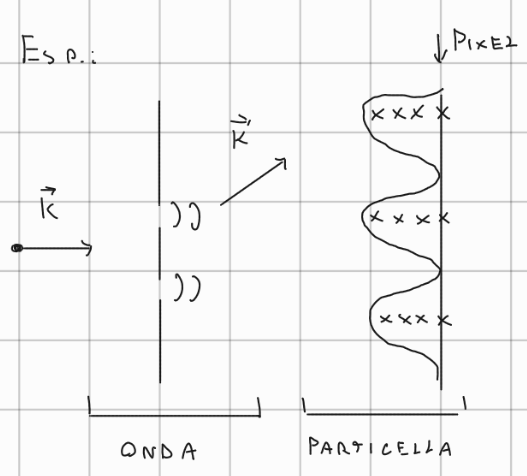
\includegraphics[width=\linewidth]{immagini/2026-03-21-15-24-32.png}
    \end{minipage}\hfill
    \begin{minipage}{0.65\textwidth}
        \textbf{Osservazioni Fondamentali:} %
        \begin{enumerate}
            \item Quando invio 1 fotone, si accende \textbf{un solo pixel} $\Rightarrow$ il fotone lo misuro sempre \textbf{INTERO} (non si divide) %.
            \item Il fotone, interagendo con le fenditure, deve acquisire nuove componenti del vettore $\vec{K}$ (altrimenti andrebbe dritto rispetto alle fenditure, senza deviare) %.
        \end{enumerate}
    \end{minipage}
\end{figure}

\noindent
\textbf{Conclusione Logica:} %
Il fotone DEVE per forza interferire in qualche modo per creare i minimi e i massimi. Poiché viaggia da solo, deve comportarsi come un'onda (che è definita contemporaneamente in tutto lo spazio) e passare da entrambe le fenditure. %
$\Rightarrow$ \textbf{IL FOTONE INTERFERISCE CON SE STESSO} %

La luce è intrinsecamente \textbf{SIA ONDA CHE PARTICELLA}: %
\begin{itemize}
    \item Quando la \textbf{MISURO} $\Rightarrow$ collassa e si manifesta come \textbf{PARTICELLA} (impatto sul pixel) %.
    \item \textbf{DURANTE IL TRAGITTO} $\Rightarrow$ si propaga come \textbf{ONDA} (Esperimento di Young) ma può interagire come \textbf{PARTICELLA} (Effetto Compton) %.
\end{itemize}

\section{Principio di Complementarietà di Bohr} %

\textbf{Definizione:} Il tipo di esperimento determina il MODELLO (ondulatorio o corpuscolare) che devo usare per descrivere il fenomeno. I due modelli sono tipicamente mutuamente esclusivi.

\begin{figure}[H]
    \centering
    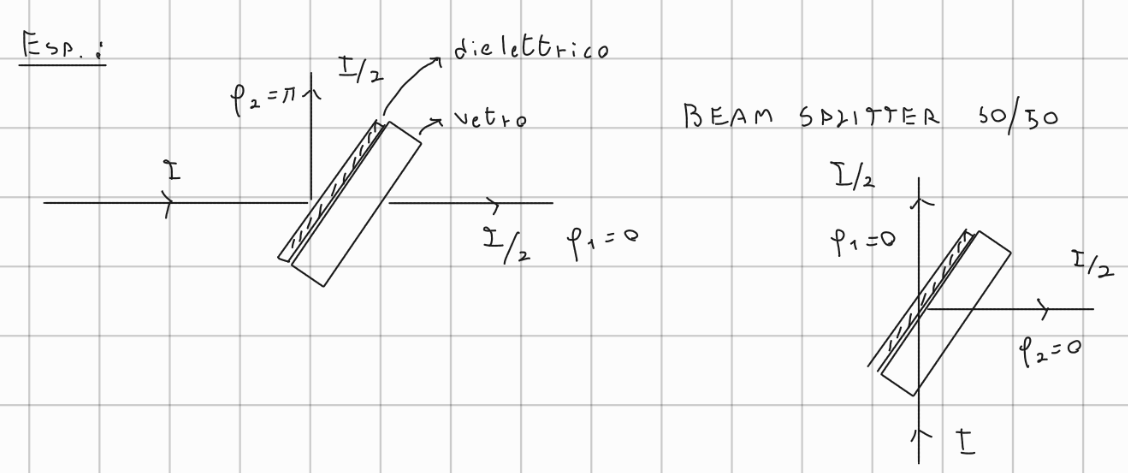
\includegraphics[width=0.6\linewidth]{immagini/2026-03-21-15-27-35.png}
    \end{figure}

\subsection{1. Esperimento con Beam Splitter (BS)} %

Consideriamo uno specchio semiriflettente (Beam Splitter 50/50), composto da un supporto in vetro e un sottile strato dielettrico %.
Quando la luce (raggio laser di intensità $I$) incide sul BS: %
\begin{itemize}
    \item La componente riflessa dal dielettrico subisce uno sfasamento $\varphi_2 = \pi$ %.
    \item La componente trasmessa (che attraversa il vetro) non subisce sfasamento, $\varphi_1 = 0$ %.
\end{itemize}

Se usiamo un laser continuo, i due rivelatori $R_1$ e $R_2$ misureranno un'intensità costante pari a $I/2$ ciascuno %.

\begin{figure}[H]
    \centering
    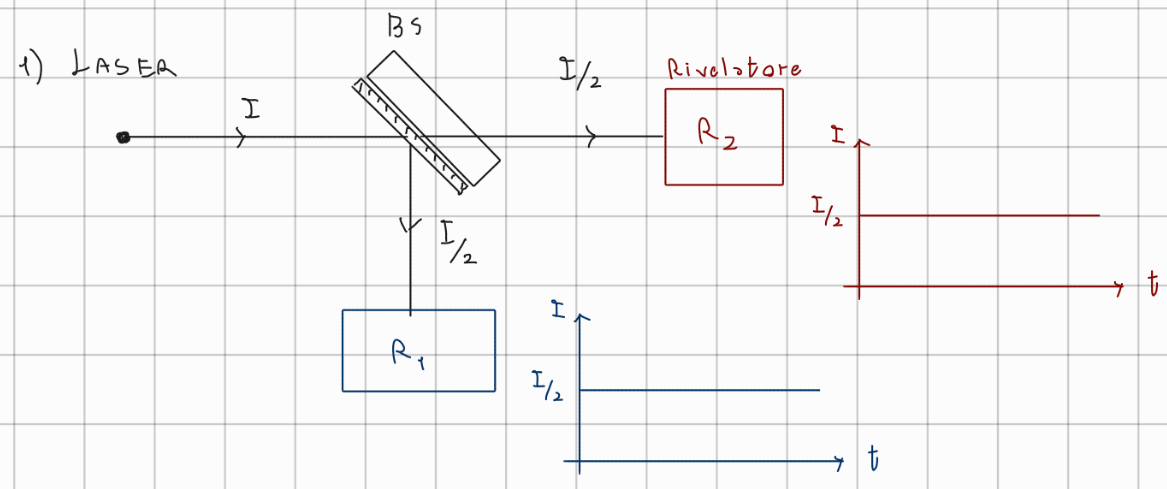
\includegraphics[width=0.6\linewidth]{immagini/2026-03-21-15-28-25.png}
    \end{figure}

\noindent
\textbf{Ora mando un fotone alla volta:} %
Se riduco l'intensità in modo da emettere singoli fotoni, i rivelatori non misurano un segnale continuo, ma registrano dei conteggi (scatti) discreti nel tempo %.
\begin{figure}[H]
    \centering
    \begin{minipage}{0.3\textwidth}
        \centering
        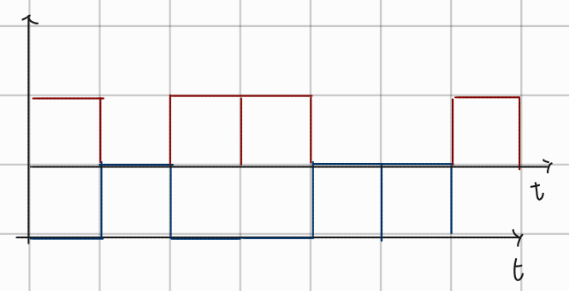
\includegraphics[width=\linewidth]{immagini/2026-03-21-15-29-10.png}
    \end{minipage}\hfill
    \begin{minipage}{0.65\textwidth}
        \begin{itemize}
            \item I rivelatori \textbf{non scattano mai insieme} nello stesso istante %.
            \item Statisticamente, il numero di conteggi su $R_1$ è uguale al numero di conteggi su $R_2$ ($50\% / 50\%$) %.
        \end{itemize}
    \end{minipage}
\end{figure}

\noindent
\textit{Conclusione:} Il fotone lo misuro sempre INTERO, in questo caso si comporta inequivocabilmente come una \textbf{PARTICELLA} %.

\subsection{2. Interferometro di Mach-Zehnder} %

Aggiungiamo degli specchi per ricombinare i due fasci separati dal primo BS facendoli incidere su un secondo BS, per poi misurarli con i rivelatori $R_1$ e $R_2$ %.

\begin{figure}[H]
    \centering
    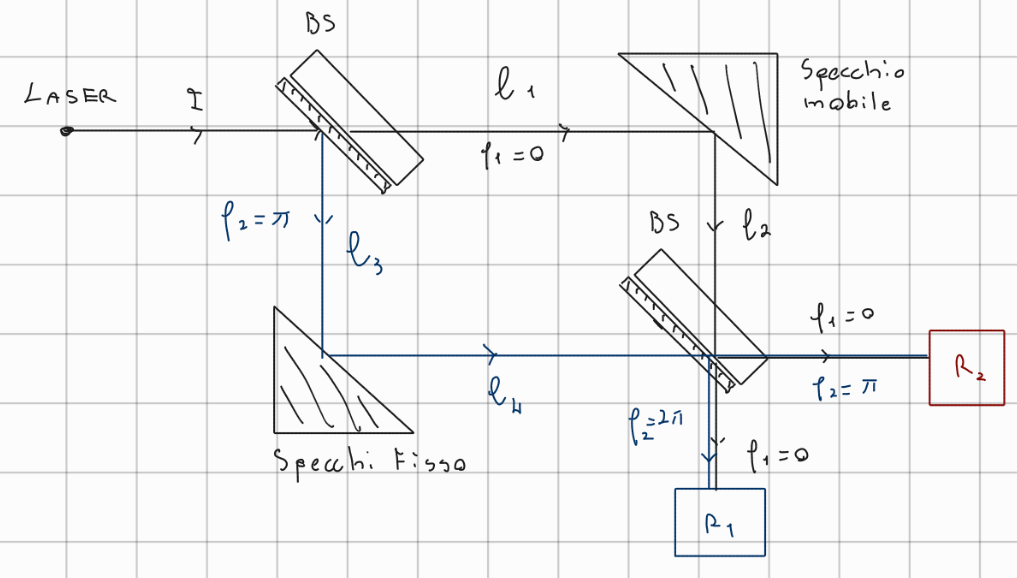
\includegraphics[width=0.5\linewidth]{immagini/2026-03-21-15-30-43.png}
    \end{figure}

\noindent
Calcoliamo le fasi totali accumulate dalla luce lungo i due percorsi per raggiungere ciascun rivelatore, sommando le fasi geometriche $k \cdot l$ e gli sfasamenti delle riflessioni %.

\textbf{Fasi al rivelatore $\mathbf{R_1}$:} %
\begin{equation}
    \begin{cases}
        \varphi_1^{tot} = k(l_1 + l_2) \\ %
        \varphi_2^{tot} = k(l_3 + l_4) + 2\pi %
    \end{cases} \quad \Rightarrow \quad \Delta\varphi_{R1} = k(l_3 + l_4 - l_1 - l_2) + 2\pi %
\end{equation}

\textbf{Fasi al rivelatore $\mathbf{R_2}$:} %
\begin{equation}
    \begin{cases}
        \varphi_1^{tot} = k(l_1 + l_2) \\ %
        \varphi_2^{tot} = k(l_3 + l_4) + \pi %
    \end{cases} \quad \Rightarrow \quad \Delta\varphi_{R2} = k(l_3 + l_4 - l_1 - l_2) + \pi %
\end{equation}

\subsection{Analisi dei casi (Onda Continua)} %

\textbf{Caso A: Cammini ottici uguali} %
Se regoliamo lo specchio mobile in modo che la differenza di cammino geometrico sia nulla: $k(l_3 + l_4 - l_1 - l_2) = 0$ %.
\begin{figure}[H]
    \centering
    \begin{minipage}{0.3\textwidth}
        \centering
        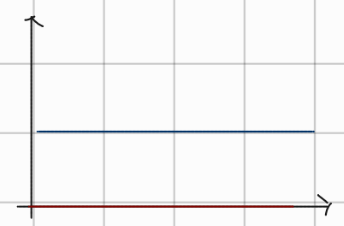
\includegraphics[width=\linewidth]{immagini/2026-03-21-15-31-41.png}
    \end{minipage}\hfill
    \begin{minipage}{0.65\textwidth}
        \begin{itemize}
            \item $\Delta\varphi_{R1} = 2\pi \quad \rightarrow \quad \text{\textbf{Interferenza Costruttiva}}$ (Massimo) %
            \item $\Delta\varphi_{R2} = \pi \quad \rightarrow \quad \text{\textbf{Interferenza Distruttiva}}$ (Minimo) %
        \end{itemize}
    \end{minipage}
\end{figure}
Tutta la luce esce verso $R_1$, mentre $R_2$ rimane completamente buio %.

\noindent
\textbf{Caso B: Spostamento di mezza lunghezza d'onda} %
Se muoviamo lo specchio in modo da introdurre un ritardo di fase geometrica pari a $\pi$: $k(l_3 + l_4 - l_1 - l_2) = \pi$ %.
\begin{figure}[H]
    \centering
    \begin{minipage}{0.3\textwidth}
        \centering
        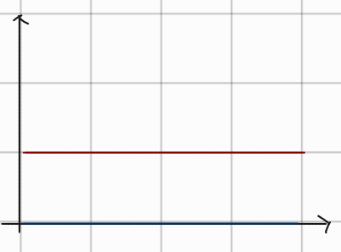
\includegraphics[width=\linewidth]{immagini/2026-03-21-15-32-00.png}
    \end{minipage}\hfill
    \begin{minipage}{0.65\textwidth}
        \begin{itemize}
            \item $\Delta\varphi_{R1} = \pi + 2\pi = 3\pi \quad \rightarrow \quad \text{\textbf{Interferenza Distruttiva}}$ %
            \item $\Delta\varphi_{R2} = \pi + \pi = 2\pi \quad \rightarrow \quad \text{\textbf{Interferenza Costruttiva}}$ %
        \end{itemize}
    \end{minipage}
\end{figure}
La situazione si ribalta: tutta la luce finisce in $R_2$ e $R_1$ è buio %.

\subsection{Analisi a Singolo Fotone (Paradosso Quantistico)} %

\textbf{ORA INVIO SOLO 1 FOTONE alla volta nell'interferometro settato come nel "Caso A".} %
\begin{figure}[H]
    \centering
    \begin{minipage}{0.3\textwidth}
        \centering
        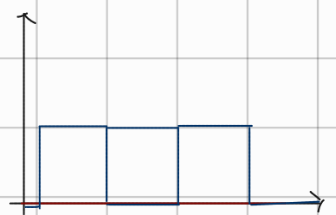
\includegraphics[width=\linewidth]{immagini/2026-03-21-15-33-15.png}
    \end{minipage}\hfill
    \begin{minipage}{0.65\textwidth}
        \begin{itemize}
            \item Sperimentalmente: \textbf{ARRIVANO TUTTI A $\mathbf{R_1}$} %.
            \item Ma per decidere di andare tutto su $R_1$ e cancellarsi su $R_2$, il fotone \textit{deve} aver "subìto" l'interferenza costruttiva e distruttiva generate dai due percorsi separati. Se fosse solo una pallina e scegliesse un ramo solo al primo BS, alla fine i rivelatori segnerebbero 50/50.
        \end{itemize}
    \end{minipage}
\end{figure}

\noindent
Ciò significa che il singolo fotone è \textbf{DELOCALIZZATO}: si trova in due punti diversi nello stesso momento per poter interferire con se stesso all'uscita %.
\begin{quote}
    \textit{Controprova:} SE BLOCCO UNA DELLE DUE STRADE, distruggo l'interferenza e TORNO A VEDERE 50/50 tra i due rivelatori! %
\end{quote}

\begin{figure}[H]
    \centering
    \begin{minipage}{0.3\textwidth}
        \centering
        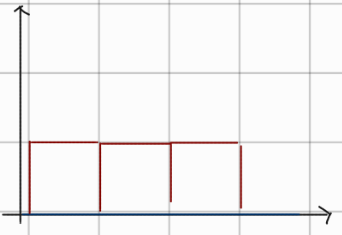
\includegraphics[width=\linewidth]{immagini/2026-03-21-15-37-43.png}
    \end{minipage}\hfill
    \begin{minipage}{0.65\textwidth}
        Se invio un solo fotone per volta con la configurazione B ottengo lo stesso effetto di "interferenza" e arrivano tutti a R2, nonostante il fotone sia sempre uno solo!
    \end{minipage}
\end{figure}

\noindent
\textbf{Connessione Matematica:} %
Classicamente, l'intensità totale dipendeva dalla sovrapposizione dei campi: %
\begin{equation*}
    |\mathcal{E}_{tot}|^2 = |\mathcal{E}_1 + \mathcal{E}_2|^2 \propto I %
\end{equation*}
Quantisticamente, sapendo che il numero di fotoni distribuiti nello spazio segue l'intensità ($N(\theta) = N_0 P(\theta)$), la probabilità quantistica si comporta esattamente come l'intensità classica: %
\begin{equation}
    \boxed{ I \Leftrightarrow P \propto |\mathcal{E}_1 + \mathcal{E}_2|^2 } %
\end{equation}
L'onda elettromagnetica diventa l'"Onda di Probabilità" che guida la particella!

\section{Dualismo Onda-Particella: Elettroni (1924, De Broglie)} %

De Broglie ipotizza che la simmetria della natura valga anche per le particelle dotate di massa %.
\begin{itemize}
    \item \textbf{Fotone:} descritto dall'onda elettromagnetica $\mathcal{E}(x,t) = \mathcal{E}_0 e^{i(kx - \omega t)}$ %.
    \item \textbf{Particelle:} devono essere descritte da un'onda di materia $\psi(x,t) = A e^{i(kx - \omega t)}$ %.
\end{itemize}

Estendendo l'ipotesi per una particella, l'energia e il momento sono: %
\begin{equation*}
    E = h\nu \quad \text{e} \quad p = \frac{h}{\lambda} %
\end{equation*}
Da cui si ricava la \textbf{Lunghezza d'onda di De Broglie}: %
\begin{equation}
    \boxed{ \lambda = \frac{h}{p} } \quad \text{e vettorialmente: } \vec{p} = \hbar \vec{k} = \hbar k \hat{u}_{prop} %
\end{equation}

\subsection{Confronto: Macroscopico vs Microscopico} %

\textbf{1. Granello di polvere (Macroscopico):} %
Sia $m = 3 \cdot 10^{-9} \text{ kg}$ e $v = 2 \cdot 10^{-2} \text{ m/s}$ %.
\begin{equation*}
    \lambda = \frac{h}{p} \simeq 10^{-23} \text{ m} %
\end{equation*}
Questo valore tende a zero ($\lambda \to 0$), essendo infinitamente più piccolo anche delle dimensioni di un atomo ($\sim 10^{-9} \text{ m}$). Affinché la polvere manifesti natura ondulatoria visibile, dovrebbe muoversi a velocità lentissime (praticamente $|\vec{v}| \simeq 10^{-21} \text{ m/s}$), ma a causa dell'agitazione termica non esiste nulla di così fermo in natura.

\noindent
\textbf{2. Elettrone (Microscopico):} %
Consideriamo un elettrone ($m_e = 9.1 \cdot 10^{-31} \text{ kg}$) accelerato con un'energia cinetica $K = 120 \text{ eV}$ %.
Poiché $K = \frac{p^2}{2m} \Rightarrow p = \sqrt{2mK}$, la lunghezza d'onda associata è: %
\begin{equation*}
    \lambda = \frac{h}{p} = \frac{h}{\sqrt{2mK}} \simeq 10^{-10} \text{ m} = 1 \text{ \AA} %
\end{equation*}
Questo $\lambda$ è paragonabile alla spaziatura atomica (corrisponde ai Raggi X), quindi \textbf{l'elettrone subirà diffrazione} attraversando un cristallo! %

\section{Diffrazione e Interferenza degli Elettroni} %

\begin{figure}[H]
    \centering
    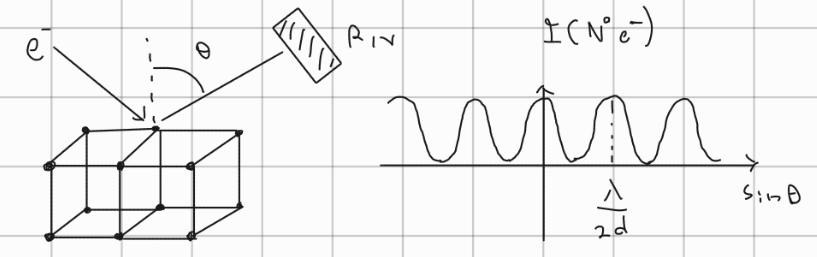
\includegraphics[width=0.5\linewidth]{immagini/2026-03-21-15-43-01.png}
    \end{figure}

Sparando elettroni su un cristallo, si osserva effettivamente un pattern di diffrazione %. 
Come per i Raggi X con la Legge di Bragg ($\sin\theta_{MAX} = m \frac{\lambda}{2d}$), si può usare il pattern misurato per stimare a ritroso la lunghezza d'onda dell'elettrone, confermando sperimentalmente che $\lambda_{e^-} \simeq 1 \text{ \AA}$ %.

\subsection{Esperimento della doppia fenditura con $\mathbf{e^-}$} %

Inviando elettroni contro una doppia fenditura, si forma un pattern di interferenza in cui l'intensità misurata sullo schermo è proporzionale al numero di elettroni incidenti ($I \propto N_{e^-}$) %.
\begin{equation}
    P \propto |\psi_{tot}|^2 = |\psi_1(\vec{r},t) + \psi_2(\vec{r},t)|^2 %
\end{equation}

\begin{figure}[H]
    \centering
    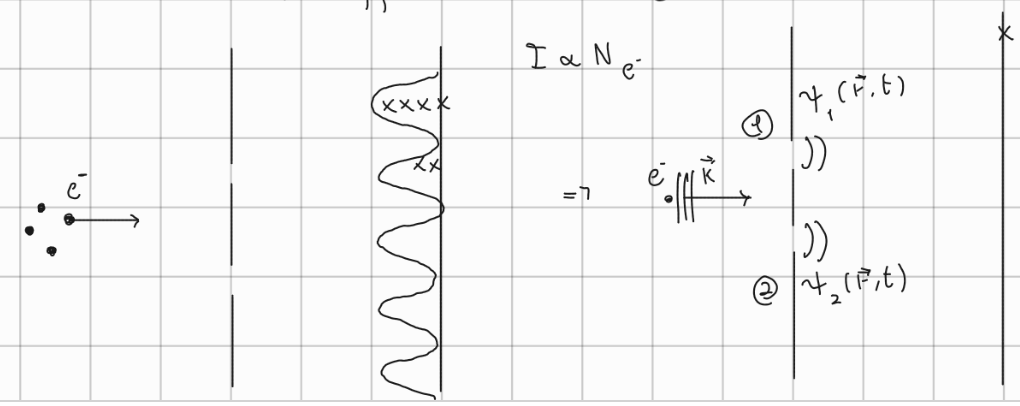
\includegraphics[width=0.6\linewidth]{immagini/2026-03-21-15-44-51.png}
    \end{figure}

\noindent
L'elettrone ha "guadagnato" componenti del vettore d'onda $\vec{k}$ che prima non aveva, diffrangendosi. % 
Diventa quindi obbligatorio \textbf{ASSOCIARE AD $\mathbf{e^-}$ UNA FUNZIONE D'ONDA} $\psi$ (le "Onde di Materia" si comportano matematicamente come $\mathcal{E}$ per la luce) %.

\begin{figure}[H]
    \centering
    \begin{minipage}{0.3\textwidth}
        \centering
        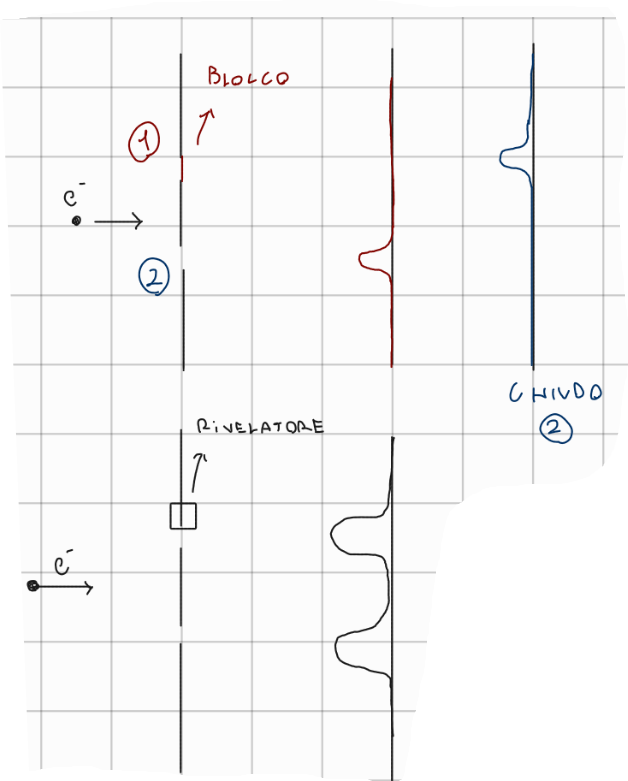
\includegraphics[width=\linewidth]{immagini/2026-03-21-15-45-42.png}
    \end{minipage}\hfill
    \begin{minipage}{0.65\textwidth}
        \begin{itemize}
            \item Se blocco una fenditura, la funzione d'onda non si sovrappone: $P \propto |\psi_1|^2$ (sparisce l'interferenza) %.
            \item Se posiziono un \textbf{RIVELATORE} per vedere da quale fenditura passa l'elettrone, costringo l'onda a collassare su una posizione definita $\Rightarrow$ \textbf{distruggo la figura d'interferenza} %.
        \end{itemize}
    \end{minipage}
\end{figure}

\section{Reinterpretazione del Modello di Bohr} %

Il dualismo onda-particella fornisce finalmente una spiegazione fisica al postulato astratto di Bohr %.
\begin{figure}[H]
    \centering
    \begin{minipage}{0.3\textwidth}
        \centering
        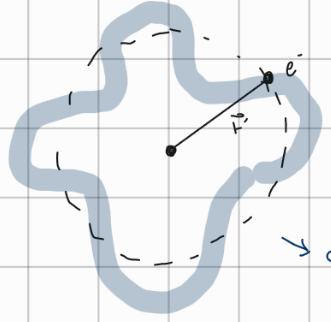
\includegraphics[width=\linewidth]{immagini/2026-03-21-15-48-11.png}
    \end{minipage}\hfill
    \begin{minipage}{0.65\textwidth}
        
        Dalla quantizzazione del momento angolare di Bohr: %
        \begin{equation*}
            L = n\hbar = n\frac{h}{2\pi} %
        \end{equation*}
        E sapendo che classicamente $L = rp$, sostituiamo il momento con la formula di De Broglie $p = \frac{h}{\lambda}$: %
        \begin{equation*}
            rp = r\frac{h}{\lambda} \quad \Rightarrow \quad n\frac{h}{2\pi} = r\frac{h}{\lambda} %
        \end{equation*}
        Semplificando $h$, otteniamo: %
        \begin{equation}
            \boxed{ n\lambda = 2\pi r } %
        \end{equation}
    \end{minipage}
\end{figure}
\noindent
Questa è la condizione geometrica affinché un'onda si chiuda perfettamente su una circonferenza senza distruggersi! %
\textit{Conclusione:} Le uniche orbite permesse per l'elettrone sono quelle in cui la sua onda di materia forma delle \textbf{ONDE STAZIONARIE} chiuse attorno al nucleo %.

\subsection{Significato Statistico della Funzione d'Onda ($\psi$)} %

\begin{figure}[H]
    \centering
    \begin{minipage}{0.25\textwidth}
        \centering
        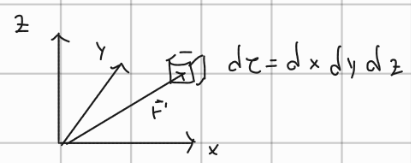
\includegraphics[width=\linewidth]{immagini/2026-03-21-15-51-24.png}
    \end{minipage}\hfill
    \begin{minipage}{0.7\textwidth}
        Consideriamo la funzione d'onda completa $\psi(\vec{r},t) = \psi(x,y,z,t)$ %.
        Definiamo un volumetto infinitesimo $d\tau = dx \, dy \, dz$ nello spazio tridimensionale %.
    \end{minipage}
\end{figure}

\noindent
Il modulo quadro della funzione d'onda $|\psi|^2$ rappresenta la \textbf{DENSITÀ DI PROBABILITÀ} %.
La probabilità $dP$ di trovare l'elettrone nel volumetto $d\tau$ all'istante $t$ è: %
\begin{equation}
    dP = |\psi(x,y,z,t)|^2 dx \, dy \, dz \quad \Rightarrow \quad P = \int_V |\psi|^2 \, d\tau %
\end{equation}

\noindent
Poiché l'elettrone deve esistere \textit{sicuramente} in qualche punto dell'intero universo (lo spazio $\mathbb{R}^3$), la probabilità totale deve essere pari a $1$. Si impone quindi la \textbf{Condizione di Normalizzazione}: %
\begin{equation}
    \boxed{ \int_{\mathbb{R}^3} |\psi|^2 \, dx \, dy \, dz = 1 } %
\end{equation}

\noindent
\textbf{Nota fisica su $\psi$:} %
Dall'integrale di normalizzazione si deduce che le dimensioni fisiche di $|\psi|^2$ sono $[|\psi|^2] = \frac{1}{\text{m}^3}$ (inverso di un volume) %.
Ne consegue che la funzione d'onda $\psi$ \textbf{NON HA SIGNIFICATO FISICO DIRETTO} misurabile. Mentre grandezze come il campo magnetico $\vec{B}$ o il campo elettrico $\vec{E}$ si misurano con gli strumenti, $\psi$ no (si misura solo il suo modulo quadro come frequenza statistica).

\section{Limiti dell'Onda Piana per le Particelle} %

\begin{figure}[H]
    \centering
    \begin{minipage}{0.25\textwidth}
        \centering
        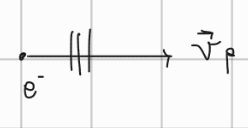
\includegraphics[width=\linewidth]{immagini/2026-03-21-15-52-48.png}
    \end{minipage}\hfill
    \begin{minipage}{0.7\textwidth}
        Proviamo a descrivere un elettrone con una semplice onda piana: %
        \begin{equation*}
            \psi(x,t) = A e^{i(kx - \omega t)} %
        \end{equation*}
    \end{minipage}
\end{figure}
Calcoliamo la sua velocità di fase $v_{onda}$: %
\begin{equation*}
    v_{onda} = \lambda \nu = \frac{h}{p} \cdot \frac{E}{h} = \frac{E}{p} = \frac{\frac{p^2}{2m}}{p} = \frac{p}{2m} = \frac{m v_p}{2m} = \frac{v_p}{2} %
\end{equation*}
(dove $v_p$ è la velocità classica della particella). %

\noindent
$\Rightarrow$ \textbf{Un'ONDA PIANA non è in grado di descrivere una particella} (viaggia alla metà della velocità attesa!). %
Un altro problema dell'onda piana è la normalizzazione, poiché l'integrale su tutto lo spazio diverge: %
\begin{equation*}
    \int_{\mathbb{R}^3} |\psi|^2 \, dx \, dy \, dz \longrightarrow +\infty \quad \text{(DIVERGE)} %
\end{equation*}

\subsection{Il Pacchetto d'Onda} %

Per descrivere una particella localizzata introduciamo il \textbf{PACCHETTO}: %
\begin{equation}
    \psi(x,t) = \frac{1}{\sqrt{2\pi}} \int_{\mathbb{R}} A(k) e^{i(kx - \omega t)} \, dk %
\end{equation}

Calcoliamo le velocità di questo pacchetto: %
\begin{itemize}
    \item \textbf{Velocità di fase ($\mathbf{v_f}$):} %
    Sapendo che $E = \frac{p^2}{2m} = \frac{\hbar^2 k^2}{2m}$: %
    \begin{equation*}
        v_f = \frac{\omega}{k} = \frac{E/\hbar}{k} = \frac{\frac{\hbar^2 k^2}{2m \hbar}}{k} = \frac{\hbar k^2}{2m k} = \frac{\hbar k}{2m} %
    \end{equation*}
    $\Rightarrow$ \textbf{DISPERDE} (ogni componente con valore di $k$ diverso viaggia a velocità diversa). %
    La \textbf{Relazione di Dispersione} è $\omega = \frac{\hbar k^2}{2m}$. %

    \item \textbf{Velocità di gruppo ($\mathbf{v_g}$):} %
    \begin{equation*}
        v_g = \frac{d\omega}{dk} = \frac{d(E/\hbar)}{d(p/\hbar)} = \frac{dE}{dp} = \frac{d}{dp}\left(\frac{p^2}{2m}\right) = \frac{2p}{2m} = \frac{p}{m} = \frac{m v_p}{m} = \underline{\underline{v_p}} %
    \end{equation*}
    \begin{figure}[H]
        \centering
        \begin{minipage}{0.3\textwidth}
            \centering
            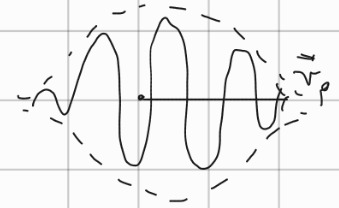
\includegraphics[width=\linewidth]{immagini/2026-03-21-15-55-53.png}
        \end{minipage}\hfill
        \begin{minipage}{0.65\textwidth}
            Il pacchetto (ovvero l'inviluppo) viaggia esattamente alla velocità della particella classica! %
        \end{minipage}
    \end{figure}
\end{itemize}

\begin{figure}[H]
    \centering
    \begin{minipage}{0.3\textwidth}
        \centering
        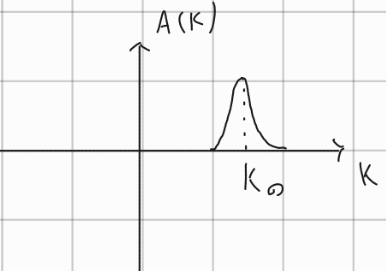
\includegraphics[width=\linewidth]{immagini/2026-03-21-15-56-15.png}
    \end{minipage}\hfill
    \begin{minipage}{0.65\textwidth}
        \noindent
        $\Rightarrow$ Da ora in poi la nostra onda piana è intesa come un pacchetto con i valori di $k$ molto vicini a un $k_0$ centrale, quasi come se il resto fosse nullo. %
    \end{minipage}
\end{figure}

\section{Significato Fisico di $\mathbf{A(k)}$} %

Discretizziamo l'integrale del pacchetto per capirne il senso fisico: %
\begin{align*}
    \psi(x,t) &= \frac{1}{\sqrt{2\pi}} \int_{\mathbb{R}} A(k) e^{i(kx - \omega t)} \, dk \quad \xrightarrow{\text{discretizzo}} \quad \sum_k A(k) e^{i(kx - \omega t)} = \\ %
    &= \underbrace{A_1(k_1)}_{\text{Numero}} e^{i(k_1 x - \omega_1 t)} + A_2(k_2) e^{i(k_2 x - \omega_2 t)} + \dots %
\end{align*}
I coefficienti $A_i$ sono semplicemente valori numerici in corrispondenza del vettore d'onda $k_i$. %

\noindent
Confrontiamo questo risultato con un'onda elettromagnetica che attraversa un prisma dispersivo: %
\begin{equation*}
    \mathcal{E} = \underbrace{\mathcal{E}_{01}}_{A_1(k_1)} e^{i(k_1 x - \omega_1 t)} + \underbrace{\mathcal{E}_{02}}_{A_2(k_2)} e^{i(k_2 x - \omega_2 t)} + \dots %
\end{equation*}

\begin{figure}[H]
    \centering
    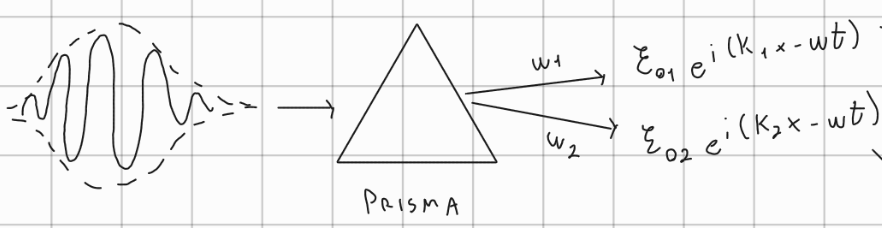
\includegraphics[width=0.6\linewidth]{immagini/2026-03-21-16-19-40.png}
    \end{figure}

Ogni singola componente ha un numero di fotoni proporzionale all'intensità: %
\begin{align*}
    N_1 \text{ fotoni} &= \frac{c \varepsilon_0 |\mathcal{E}_{01}|^2}{2\hbar\omega_1} = \frac{c \varepsilon_0 |A_1(k_1)|^2}{2\hbar\omega_1} \\ %
    N_2 \text{ fotoni} &= \frac{c \varepsilon_0 |\mathcal{E}_{02}|^2}{2\hbar\omega_2} = \frac{c \varepsilon_0 |A_2(k_2)|^2}{2\hbar\omega_2} %
\end{align*}
$\Rightarrow$ Più l'ampiezza $A(k)$ è grande $\Rightarrow$ più è grande il numero di fotoni presenti con quel preciso vettore d'onda $k$. %
Di conseguenza, il modulo quadro dell'ampiezza $|A(k)|^2$ fornisce la \textbf{probabilità} $P$ di avere un fotone nel range tra $k$ e $k+dk$. %

\subsection{Confronto Probabilistico: Fotoni vs Elettroni} %

\textbf{FOTONI (Luce):} %
\begin{itemize}
    \item Nello spazio dei momenti: $\boxed{ |A(k)|^2 dk = P }$ (Probabilità di avere un fotone con vettore d'onda compreso tra $k$ e $k+dk$). %
    $\Rightarrow$ Rappresenta una vera e propria \textbf{DENSITÀ DI PROBABILITÀ}, dove $A(k)$ è l'ampiezza di ogni componente del pacchetto. %
    \item Nello spazio reale: l'espressione $|\mathcal{E}|^2 d\tau$ per trovare un fotone nel volume $d\tau$ \textbf{NON è vero}. A causa dei principi della relatività (in qualsiasi sistema di riferimento il fotone viaggia sempre a velocità $c$), non si può definire una probabilità di localizzazione statica del fotone.
    $\Rightarrow$ Di conseguenza, $A(k)$ agisce di fatto come la "funzione d'onda" del fotone nello spazio dei momenti. %
\end{itemize}

\noindent
\textbf{ELETTRONI (o Particelle dotate di massa):} %
A differenza del fotone, per le particelle massive esistono entrambe le descrizioni probabilistiche, che sono complementari: %
\begin{itemize}
    \item Nello spazio dei momenti: $|A(k)|^2 dk = P$ (Prob. di avere un elettrone con vettore d'onda $k \div k+dk$, ovvero con quantità di moto $p \div p+dp$). %
    \item Nello spazio reale: $|\psi|^2 d\tau = P$ (Prob. di trovare un elettrone fisicamente localizzato nel volumetto $d\tau$). %
\end{itemize}

\section{Principio (di Indeterminazione) di Heisenberg} %

Sia $p_0 = \hbar k_0$ il momento medio di un pacchetto d'onda. %
Consideriamo un'ampiezza di probabilità nello spazio dei momenti distribuita come una \textbf{Gaussiana}: %
\begin{figure}[H]
    \centering
    \begin{minipage}{0.3\textwidth}
        \centering
        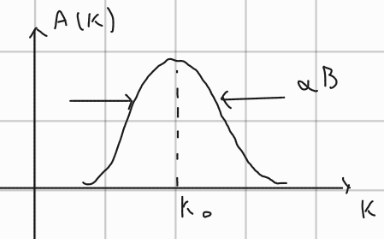
\includegraphics[width=\linewidth]{immagini/2026-03-21-16-26-09.png}
    \end{minipage}\hfill
    \begin{minipage}{0.65\textwidth}
        \begin{equation}
            A(k) = c e^{-\frac{(k-k_0)^2}{2B^2}} %
        \end{equation}
    \end{minipage}
\end{figure}
dove $B$ è proporzionale alla larghezza della campana centrata in $k_0$. %

Calcoliamo la funzione d'onda nello spazio delle posizioni a $t=0$: %
\begin{align*}
    \psi(x,0) &= \frac{1}{\sqrt{2\pi}} \int_{\mathbb{R}} A(k) e^{ikx} \, dk = \underbrace{\frac{c}{\sqrt{2\pi}}}_{c'} \int_{\mathbb{R}} e^{-\frac{(k-k_0)^2}{2B^2}} e^{ikx} \, dk %
\end{align*}

Applichiamo la sostituzione $q = k - k_0 \Rightarrow dk = dq$: %
\begin{align*}
    \psi(x,0) &= c' \int_{\mathbb{R}} e^{-\frac{q^2}{2B^2}} e^{i(q+k_0)x} \, dq = c' e^{ik_0 x} \int_{\mathbb{R}} e^{-\frac{q^2}{2B^2}} e^{iqx} \, dq = \\ %
    &= c' e^{ik_0 x} \int_{\mathbb{R}} e^{-\left[ \frac{q^2}{2B^2} - iqx \right]} \, dq %
\end{align*}

Completiamo il quadrato all'esponente: %
\begin{equation*}
    \frac{q^2}{2B^2} - iqx = \frac{q^2 - iqx(2B^2)}{2B^2} = \frac{q^2 - 2iqxB^2}{2B^2} - \frac{x^2 B^4}{2B^2} + \frac{x^2 B^2}{2} = \left[ \frac{q}{\sqrt{2}B} - \frac{ixB}{\sqrt{2}} \right]^2 + \frac{x^2 B^2}{2} %
\end{equation*}

Sostituendo nell'integrale: %
\begin{align*}
    \psi(x,0) &= c' e^{ik_0 x} \int_{\mathbb{R}} e^{-\left( \frac{q}{\sqrt{2}B} - \frac{ixB}{\sqrt{2}} \right)^2 - \frac{x^2 B^2}{2}} \, dq = c' e^{ik_0 x} e^{-\frac{x^2 B^2}{2}} \int_{\mathbb{R}} e^{-\left( \frac{q}{\sqrt{2}B} - \frac{ixB}{\sqrt{2}} \right)^2} \, dq %
\end{align*}

Definiamo $u = \frac{q}{\sqrt{2}B} - \frac{ixB}{\sqrt{2}} \Rightarrow du = \frac{dq}{\sqrt{2}B} \Rightarrow dq = \sqrt{2}B \, du$: %
\begin{align*}
    \psi(x,0) &= c' e^{ik_0 x} e^{-\frac{x^2 B^2}{2}} \int_{\mathbb{R}} \sqrt{2}B e^{-u^2} \, du = \underbrace{\sqrt{2\pi} B c'}_{c''} e^{ik_0 x} e^{-\frac{x^2 B^2}{2}} %
\end{align*}

Scrivendolo in forma canonica gaussiana, otteniamo l'onda piana modulata dal pacchetto: %
\begin{equation}
    \boxed{ \psi(x,0) = c'' e^{ik_0 x} e^{-\frac{x^2}{2(1/B)^2}} } %
\end{equation}

\subsection{Varianza e Incertezza ($\Delta x$ e $\Delta k$)} %

Analizziamo le deviazioni standard (incertezze) delle probabilità $|A(k)|^2$ e $|\psi(x,0)|^2$: %
\begin{align*}
    |A(k)|^2 &= |c|^2 e^{-\frac{(k-k_0)^2}{B^2/2}} \quad \Rightarrow \quad 2\sigma_k^2 = B^2 \quad \Rightarrow \quad \sigma_k = \frac{B}{\sqrt{2}} \\ %
    |\psi(x,0)|^2 &= |c''|^2 e^{-\frac{x^2}{1/B^2}} \quad \Rightarrow \quad 2\sigma_x^2 = \frac{1}{B^2} \quad \Rightarrow \quad \sigma_x = \frac{1}{\sqrt{2}B} %
\end{align*}

Moltiplicando le due deviazioni standard, il parametro $B$ si semplifica: %
\begin{equation}
    \sigma_k \sigma_x = \left(\frac{B}{\sqrt{2}}\right) \left(\frac{1}{\sqrt{2}B}\right) = \frac{1}{2} %
\end{equation}
\begin{figure}[H]
    \centering
    \begin{minipage}{0.4\textwidth}
        \centering
        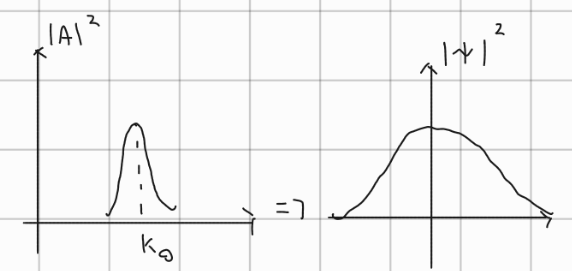
\includegraphics[width=\linewidth]{immagini/2026-03-21-16-32-19.png}
    \end{minipage}\hfill
    \begin{minipage}{0.55\textwidth}
        Questo dimostra matematicamente che: se "allargo" $A(k)$, necessariamente "stringo" $\psi$ e viceversa. %
    \end{minipage}
\end{figure}

\noindent
Identificando le deviazioni standard con le \textbf{Incertezze} ($\sigma_k = \Delta k$ e $\sigma_x = \Delta x$): %
\begin{equation*}
    \Delta k \Delta x = \frac{1}{2} \quad \text{(pacchetto gaussiano a } t=0) %
\end{equation*}
Poiché $p = \hbar k \Rightarrow \Delta p = \hbar \Delta k$ (l'incertezza sul momento è legata a quella sul vettore d'onda): %
\begin{equation}
    \boxed{ \Delta p \Delta x = \frac{\hbar}{2} } %
\end{equation}

\subsection{Evoluzione Temporale ($t>0$)} %

Cosa succede per tempi positivi? %
La fase temporale è $\omega t = \frac{E t}{\hbar} = \frac{1}{\hbar} \frac{\hbar^2 k^2}{2m} t = \frac{\hbar k^2}{2m} t$. %
La funzione d'onda nel tempo diventa: %
\begin{equation*}
    \psi(x,t) = \frac{1}{\sqrt{2\pi}} \int_{\mathbb{R}} A(k) e^{i\left(kx - \frac{\hbar k^2}{2m}t\right)} \, dk %
\end{equation*}

\noindent
Calcolando questo integrale per un pacchetto gaussiano, si ottiene che l'incertezza sulla posizione $\sigma_x$ \textbf{aumenta nel tempo}: %
\begin{equation}
    \sigma_x(t) = \sigma_0 [1 + f(t)] \quad \rightarrow \quad \text{MONOTONA CRESCENTE} %
\end{equation}

\begin{figure}[H]
    \centering
    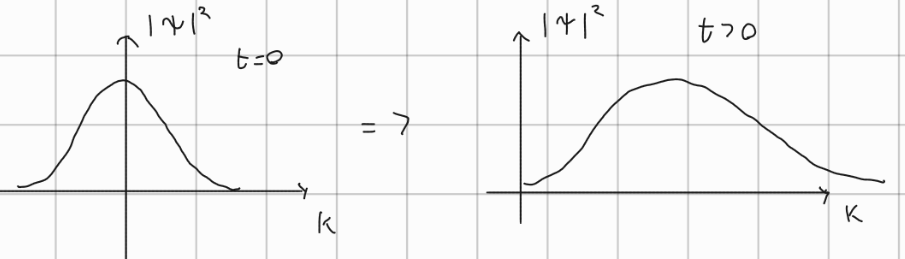
\includegraphics[width=0.6\linewidth]{immagini/2026-03-21-16-34-30.png}
    \end{figure}

\noindent
Pertanto, la relazione $\Delta x \Delta k = 1/2$ è un limite inferiore assoluto raggiunto solo dal pacchetto gaussiano a $t=0$. %

\subsection{Definizione Generale delle Incertezze} %

Isoliamo le dipendenze spaziali e temporali della funzione d'onda: %
\begin{align*}
    f(x,t) \quad &\rightarrow \quad f(x) = f(x,0) \\ %
                 &\rightarrow \quad f(t) = f(0,t) %
\end{align*}

Le coppie di trasformate (diretta e inversa) che legano le grandezze coniugate sono: %

\textbf{1. Dominio Spaziale (Posizione $x$ e Vettore d'onda $k$):} %
\begin{equation}
    f(x) = \frac{1}{\sqrt{2\pi}} \int_{\mathbb{R}} A(k) e^{ikx} \, dk \quad \rightleftarrows \quad A(k) = \frac{1}{\sqrt{2\pi}} \int_{\mathbb{R}} f(x) e^{-ikx} \, dx %
\end{equation}

\textbf{2. Dominio Temporale (Tempo $t$ e Pulsazione $\omega$):} %
\begin{equation}
    f(t) = \frac{1}{\sqrt{2\pi}} \int_{\mathbb{R}} G(\omega) e^{i\omega t} \, d\omega \quad \rightleftarrows \quad G(\omega) = \frac{1}{\sqrt{2\pi}} \int_{\mathbb{R}} f(t) e^{-i\omega t} \, dt %
\end{equation}

% --- FINE BLOCCO ---

Per una generica funzione d'onda $f(x)$ o $f(t)$, si definisce il centro della distribuzione (Media): %
\begin{align*}
    \langle x \rangle &= \frac{\int_{\mathbb{R}} x |f(x)|^2 \, dx}{\int_{\mathbb{R}} |f(x)|^2 \, dx} & \langle k \rangle &= \frac{\int_{\mathbb{R}} k |A(k)|^2 \, dk}{\int_{\mathbb{R}} |A(k)|^2 \, dk} %
\end{align*}

E l'incertezza $\Delta x$ (o Deviazione Standard $\sigma_x$) è definita come: %
\begin{equation}
    \Delta x = \sigma_x = \sqrt{ \frac{\int_{\mathbb{R}} (x - \langle x \rangle)^2 |f(x)|^2 \, dx}{\int_{\mathbb{R}} |f(x)|^2 \, dx} } \quad \text{(Stessa cosa per } \Delta k \text{)} %
\end{equation}

\noindent
Per \textbf{qualsiasi} forma del pacchetto, la disuguaglianza di Cauchy-Schwarz ($|\vec{u} \cdot \vec{v}| \le ||\vec{u}|| \cdot ||\vec{v}||$) applicata agli operatori posizione e momento garantisce che: %
\begin{equation*}
    \Delta x \Delta k \ge \frac{1}{2} \quad \text{e analogamente per tempo-frequenza} \quad \Delta \omega \Delta t \ge \frac{1}{2} %
\end{equation*}

\noindent
Essendo $k = \frac{p}{\hbar}$ e $\omega = \frac{E}{\hbar}$, otteniamo la forma finale del \textbf{Principio di Indeterminazione di Heisenberg} (Conseguenza diretta del formalismo di Fourier): %
\begin{equation}
    \boxed{ \Delta x \Delta p \ge \frac{\hbar}{2} } \qquad \text{e} \qquad \boxed{ \Delta E \Delta t \ge \frac{\hbar}{2} } %
\end{equation}

\subsection{Significato Statistico (L'Ensemble)} %

Le grandezze $\Delta x$ e $\Delta p$ sono grandezze statistiche ben definite: l'incertezza coincide con la deviazione standard ($\Delta = \sigma$) %.
Se conosco esattamente la posizione $x$, $\Delta x$ tende a $0$, costringendo l'incertezza sul momento $\Delta p$ a divergere verso l'infinito ($\Delta p \to \infty$) per rispettare la disequazione %.

\noindent
Per ottenere la deviazione standard, devo fare un altissimo numero di misurazioni identiche. Ciò richiede un \textbf{ENSEMBLE}:
Preparando $2N$ sistemi (scatole) identici: %
\begin{itemize}
    \item Su $N$ sistemi misuro la posizione $x$ $\Rightarrow$ Ottengo un certo $\Delta x$ (es. molto piccolo se la scatola è stretta) %.
    \item Sui restanti $N$ sistemi misuro la velocità $\Rightarrow p = mv \Rightarrow$ Troverò un $\Delta p$ che, moltiplicato per il $\Delta x$ precedente, obbedisce a $\Delta x \Delta p \ge \hbar/2$ %.
\end{itemize}





\end{document}